\documentclass{article}

\usepackage{graphicx}
\usepackage{tikz}
\usepackage{tikzsymbols}
\usetikzlibrary{calc,patterns,shapes.geometric}
\pagestyle{empty}
\usepackage[margin=0pt]{geometry}
\geometry{papersize={14in,12in}}

\def\centerarc[#1](#2)(#3:#4:#5){\draw[#1] ($(#2)+({#5*cos(#3)},{#5*sin(#3)})$) arc (#3:#4:#5);}

\begin{document}
	\begin{figure}
		\centering
		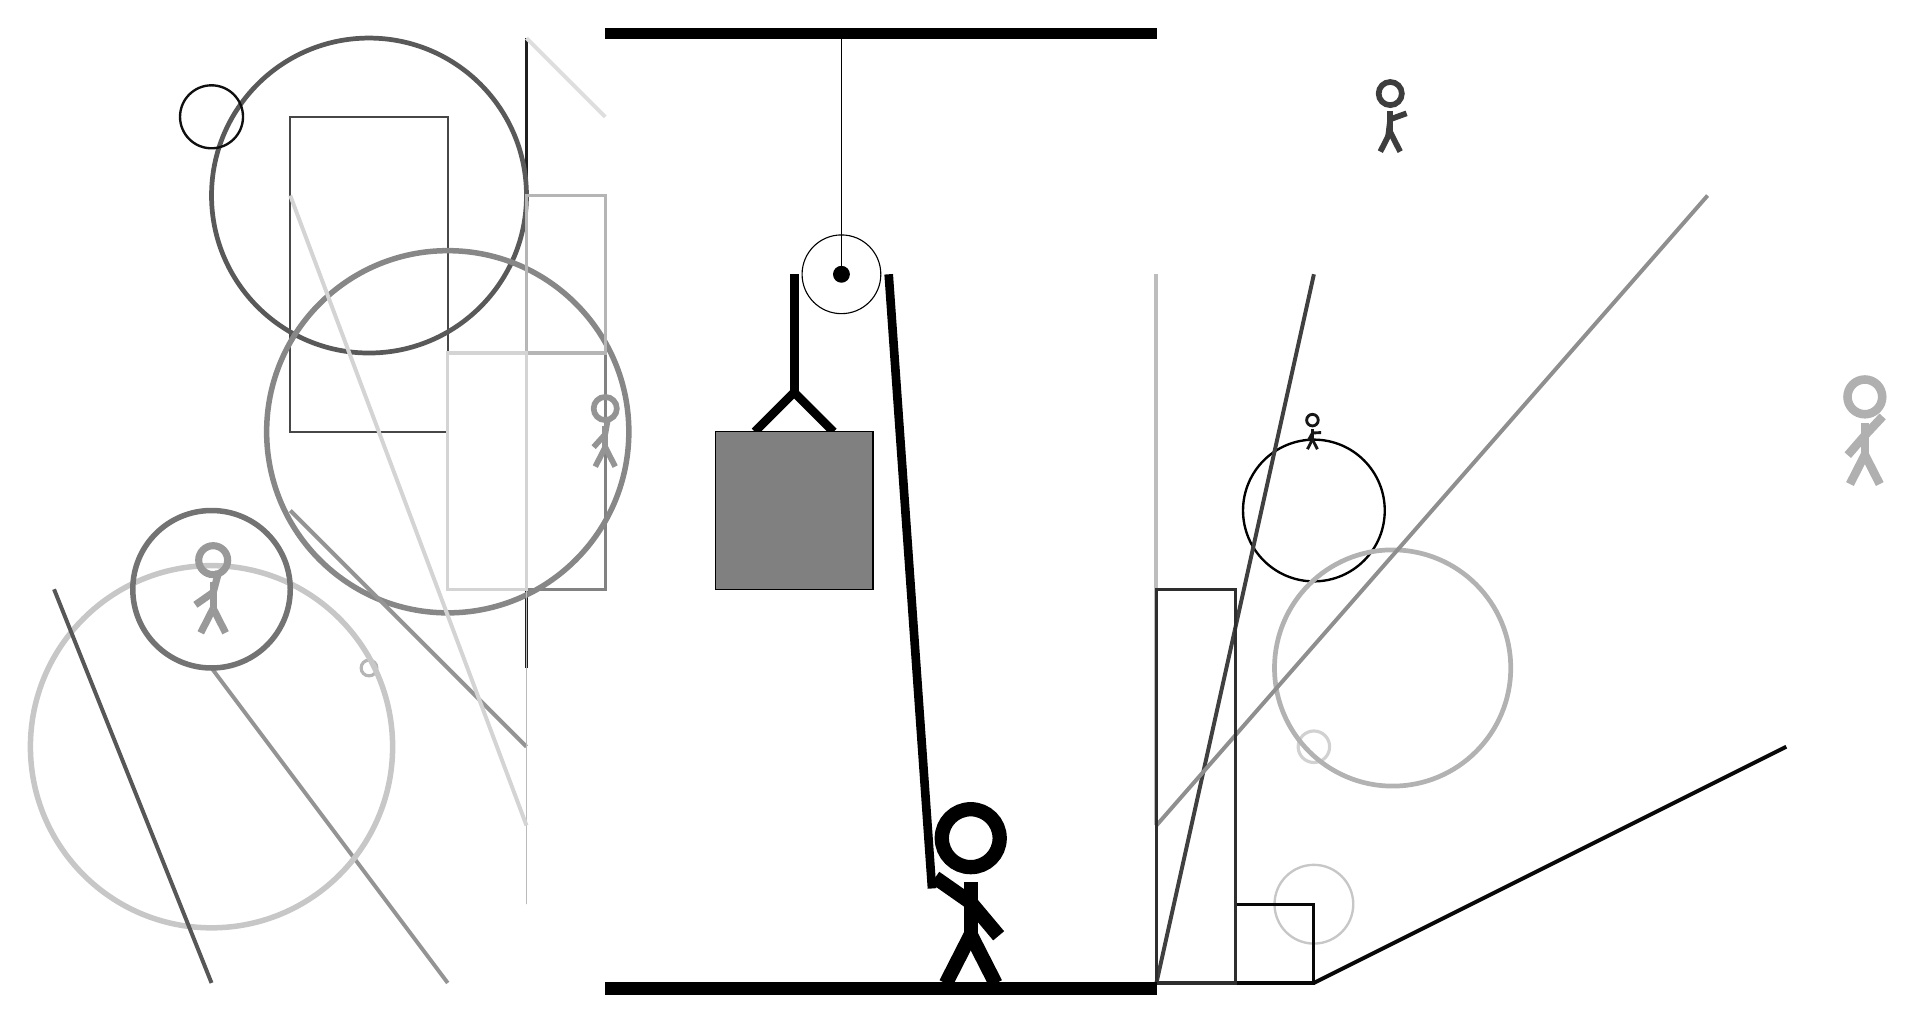
\begin{tikzpicture}
			%%%%% START %%%%%
			
			\draw[fill=black] (-2, 9) rectangle (5, 9.125);
			
			\draw (1, 6) circle (0.5);
			\draw[fill=black] (1, 6) circle (0.1);
			\draw (1, 9) -- (1, 6);
			
			\draw[line width=1.1mm] (-0.1, 4.0) -- (0.4, 4.5) -- (0.9, 4.0);
			\draw[fill=black!50] (-0.6, 4.0) rectangle (1.4, 2.0);
			
			\draw[line width=0.5mm, color=black!97](7, -3) -- (13, 0);
			
			\draw[line width=0.5mm, color=black!42](-7, 1) -- (-4, -3);
			\draw[line width=0.3mm, color=black!72] (-4, 8) rectangle (-6, 4);
			\draw[line width=0.3mm, color=black!66] (-3, 3) rectangle (-3, 8);
			\draw [line width=0.4mm, color=black!18](7, 0) circle (0.2);
			\draw[line width=0.4mm, color=black!49] (-3, 5) rectangle (-2, 2);
			\draw[line width=0.4mm, color=black!88] (-3, 1) rectangle (-3, 9);
			\draw [line width=0.3mm, color=black!100](7, 3) circle (0.9);
			\draw [line width=0.4mm, color=black!29](-5, 1) circle (0.1);
			
			\draw [line width=0.6mm, color=black!65](-5, 7) circle (2.0);
			\draw [line width=0.7mm, color=black!22](-7, 0) circle (2.3);
			\draw [line width=0.6mm, color=black!30](8, 1) circle (1.5);
			\draw [line width=0.7mm, color=black!47](-4, 4) circle (2.3);
			
			\draw[line width=0.4mm, color=black!29] (-3, 5) rectangle (-2, 7);
			\draw[line width=0.5mm, color=black!26](5, -1) -- (5, 6);
			\draw[line width=0.5mm, color=black!75](7, 6) -- (5, -3);
			
			\draw[line width=0.5mm, color=black!13](-3, 9) -- (-2, 8);
			
			\draw [line width=0.7mm, color=black!55](-7, 2) circle (1.0);
			\draw[line width=0.3mm, color=black!85] (7, 6) rectangle (7, 6);
			
			\node[line width=0.5mm, color=black!31] at (14, 4) {\Strichmaxerl[6][49][47]};
			\draw[line width=0.5mm, color=black!66](-7, -3) -- (-9, 2);
			
			\draw [line width=0.3mm, color=black!22](7, -2) circle (0.5);
			\draw[line width=0.4mm, color=black!97] (7, -2) rectangle (6, -3);
			\draw[line width=0.5mm, color=black!42](-3, 0) -- (-6, 3);
			\node[line width=0.4mm, color=black!42] at (-2, 4) {\Strichmaxerl[4][48][80]};
			\draw[line width=0.2mm, color=black!27] (-3, 6) rectangle (-3, -2);
			\draw[line width=0.4mm, color=black!17] (-4, 2) rectangle (-3, 5);
			\node[line width=0.2mm, color=black!40] at (-7, 2) {\Strichmaxerl[5][35][75]};
			\draw [line width=0.3mm, color=black!94](-7, 8) circle (0.4);
			\node[line width=0.6mm, color=black!76] at (8, 8) {\Strichmaxerl[4][83][20]};
			\node[line width=0.5mm, color=black!91] at (7, 4) {\Strichmaxerl[2][61][3]};
			
			\draw[line width=0.5mm, color=black!17](-3, -1) -- (-6, 7);
			\draw[line width=0.5mm, color=black!44](5, -1) -- (12, 7);
			\draw[line width=0.4mm, color=black!82] (6, -3) rectangle (5, 2);
			
			\draw[line width=1.1mm] (0.4, 6) -- (0.4, 4.5);
			\centerarc[line width=1.1mm](1, 6)(0:180:0.6);
			\draw[line width=1.1mm](1.6, 6) -- (2.15, -1.8);
			
			\node at (2.6, -1.9) {\Strichmaxerl[10][-35][-50]};
			
			\draw[fill=black] (-2, -3) rectangle (5, -3.15);
			
			%%%%% END %%%%%
		\end{tikzpicture}
	\end{figure}	
\end{document}